Let's test the results given by the following theorems on a sequence of uniformly refined mesh. This'll let us test the reliability and the efficiency of the error estimator $\eta$.

\subsection{Reliability}

\begin{theorem}[Reliability]
	Let $u \in H_0^1(\Omega)$ solution to the Poisson problem and $u_h$ solution to the Lagrangian FEM with a shape regular and quasi-uniform mesh $\Tau_h$. \\
	Then $\exists C$\footnote{$C$ depends only on the mesh $\Tau_h$.} such that:
	\begin{gather}
		\lvert u - u_h \rvert_{1, \Omega} \leq C \eta,
	\end{gather}
	where:
	\begin{gather}
		\eta^2 = \sum_{K \in \Tau_h} \eta_K^2.
	\end{gather}
\end{theorem}

\begin{figure}[!ht]
	\centering
	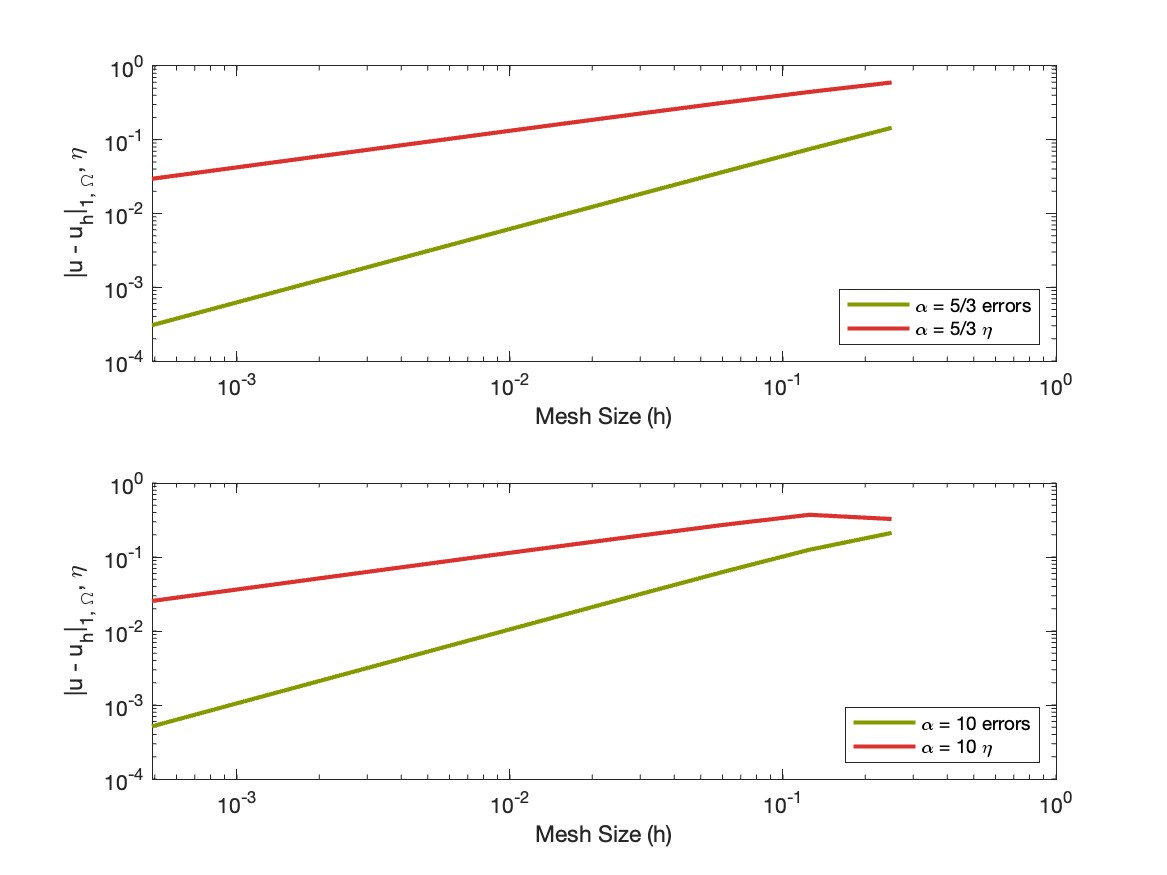
\includegraphics[width=15cm]{reliability.jpg}
	\caption{Comparison between errors and estimator against mesh size.}
\end{figure}

\newpage
\lstinputlisting{../results/reliability.txt}

\newpage
\subsection{Efficiency}

\begin{theorem}[Efficiency]
	Let $u \in H_0^1(\Omega)$ solution to the Poisson problem and $u_h$ solution to the Lagrangian FEM with a shape regular and quasi-uniform mesh $\Tau_h$. \\
	Then $\exists C$\footnote{$C$ depends on the mesh $\Tau_h$ and the FEM polynomial order $p$.} such that $\forall K \in \Tau_h$:
	\begin{gather}
		\eta_K \leq C \left[ \lvert u - u_h \rvert_{1, \omega_K} + \sum_{\tilde{K} \in \omega_K} h_{\tilde{K}} \lVert f - f_h \rVert_{0, \tilde{K}} \right].
	\end{gather}
\end{theorem}